\RequirePackage{fix-cm}
%
%\documentclass{template/svjour3}                     % onecolumn (standard format)
%\documentclass[smallcondensed]{template/svjour3}     % onecolumn (ditto)
\documentclass[smallextended]{template/svjour3}       % onecolumn (second format)
%\documentclass[twocolumn]{template/svjour3}          % twocolumn
%
\smartqed  % flush right qed marks, e.g. at end of proof
%
\usepackage{graphicx}
\usepackage{latexsym}
\usepackage{amsmath}
\usepackage{alltt}
\usepackage{amssymb}
\usepackage{chemfig}
\usepackage{mathtools}
\usepackage{listings}
\usepackage{wrapfig}
\usepackage{color}
\usepackage{float}
\usepackage{caption}
\usepackage{subcaption}
\usepackage{multicol}
\usepackage{paralist}
\usepackage{tcolorbox}
\usepackage{braket}

% Insert the name of "your journal" with
% \journalname{myjournal}

\begin{document}

\title{Energy Flow Distributions%\thanks{Grants or other notes
  %about the article that should go on the front page should be
  %placed here. General acknowledgments should be placed at the end of the article.}
}
\subtitle{Unsupervised Methods in Jet Substructure Analysis}

\author{Animesh Sinha \and Jai Bardhan \and Kalp Shah}

\authorrunning{Short form of author list} % if too long for running head

\institute{
  International Institute of Information Technology \at
  Gachibowli, Hyderabad \\
  \email{animesh.sinha@research.iiit.ac.in}
  \and
  International Institute of Information Technology \at
  Gachibowli, Hyderabad \\
  \email{jai.bardhan@research.iiit.ac.in}
  \and
  International Institute of Information Technology \at
  Gachibowli, Hyderabad \\
  \email{kalp.shah@research.iiit.ac.in}
}

\date{Submitted: \today}

\maketitle

\begin{abstract}
  In this article we present Unsupervised Machine Learning techniques on the analysis Jet Substructure using Energy Flow Polynomials as the method of choice for jet representation. We evaluate the distribution of these polynomials over different kinds of jets. These distributions are used for unsupervised probabilisitic tagging Boosted Top jets and show improved accuracy over other unsupervised techniques. Finally, we discuss anomaly detection and model-free searches for new Physics by augmenting Energy Flow Polynomials with the particle level constituents.
  \keywords{Jet Substructure \and Energy Flow \and Jet Tagging}
\end{abstract}

\section{Introduction}
\label{sec:intro}

The use of Machine Learning in attempts to find new physics by probing High Energy Particle interactions has been ubiquitous, but unsupervised techiques are yet to find their place in this landscape. With vast volumes of data available from experiments like the Large Hadron Collider (LHC), it becomes increasingly desirable and ever more plausible that Unsupervised and Model-Free learning take a leading role in the hunt for new Physics.

Jet substructure is the analysis of radiation patterns and particle distributions within the collimated sprays of particles (jets) emerging from high-energy collisions. \cite{energyflow_poly}.
It has found a central importance in many of the searches for new physics at the Large Hadron Collider (LHC) and otherwise, some of them being:
\begin{itemize}
    \item Standard Model measurements
    \item Identification of boosted heavyparticles
    \item Discrimination of quark- from gluon- initiated jets
    \item Search of Beyond Standard Model particles
\end{itemize}

\subsection{Energy Flow Polynomials (EFPs)}

We have had several methods to represent jets as inputs to computational models, from a list of 4-vectors of constituent particles, to images of the jet itself amongst others, but either they are extremely sparse representations of the jets (as in the images) making is hard to ML models to learn something meaningful, or they have had an ordering (as in lists) not providing permutation invariance.

\begin{figure}
    \centering
    \begin{subfigure}[b]{0.49\textwidth}
        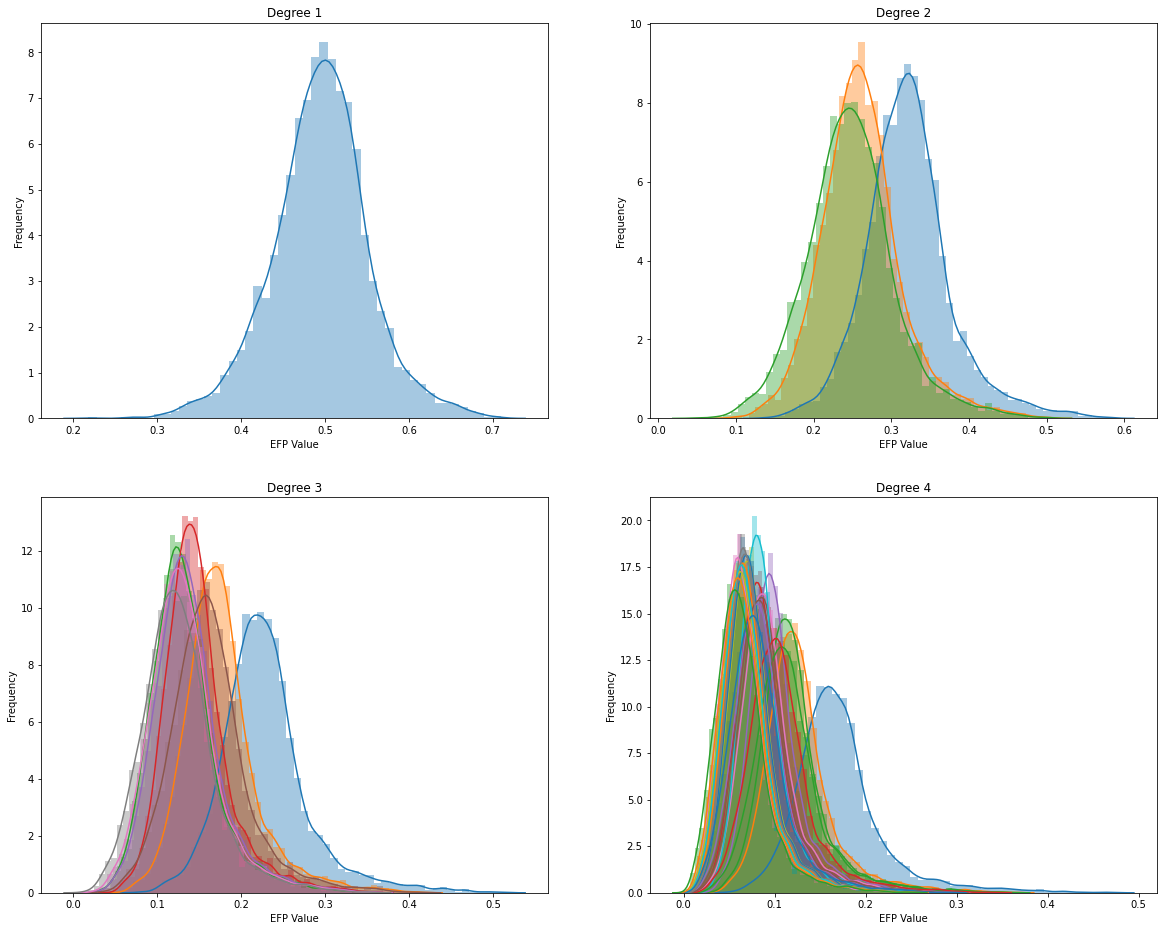
\includegraphics[width=\textwidth]{img/efp-qcd-particlenetdata.png}
        \caption{Histograms for QCD Jets}
    \end{subfigure}
    \begin{subfigure}[b]{0.49\textwidth}
        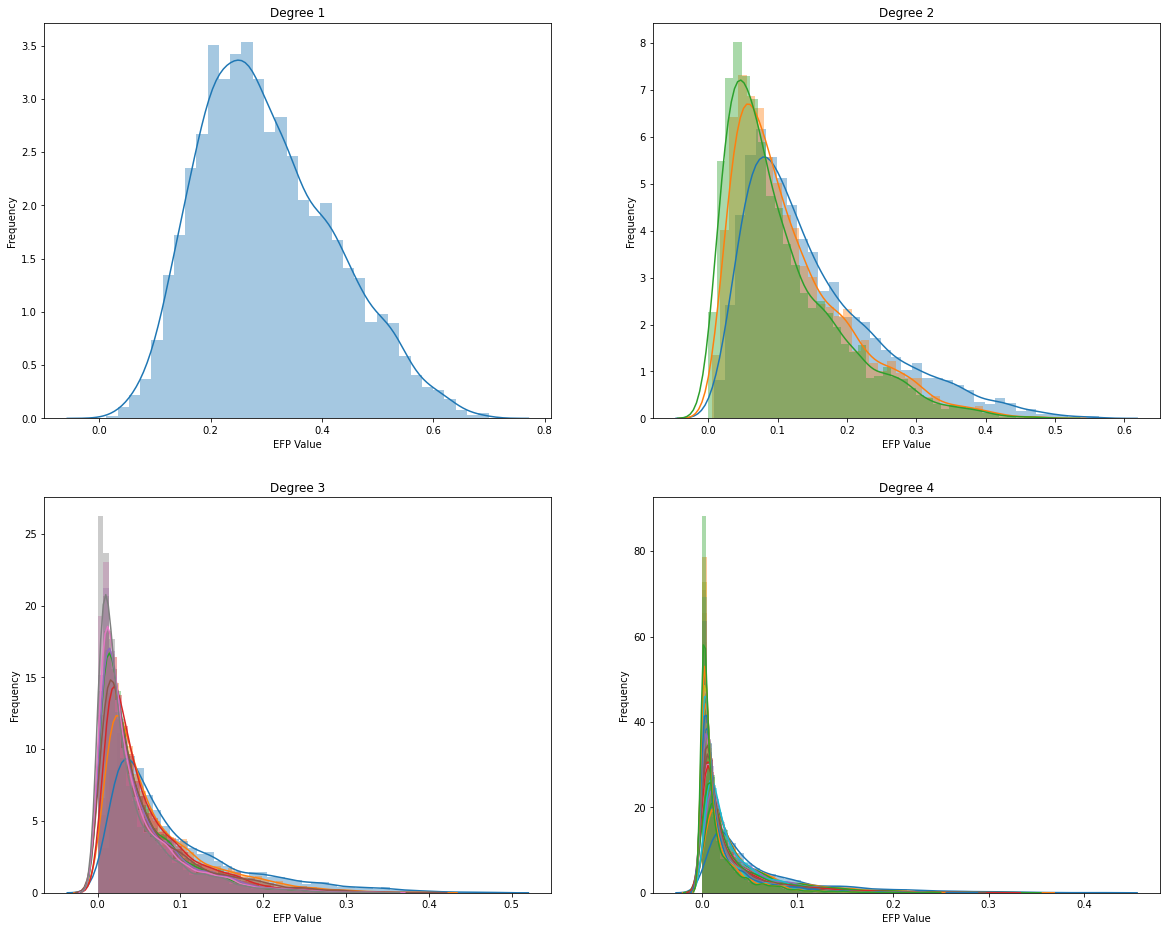
\includegraphics[width=\textwidth]{img/efp-top-particlenetdata.png}
        \caption{Histograms for Top Jets}
    \end{subfigure}
    \caption{EFP Polynomials on Top Tagging data}
    \label{fig:efp-histogram}
\end{figure}

\paragraph{EFPs as a method of jet representation} are both dense representations which inherently have permutation, as well as translational and rotational invariance. For any given jet, it's EFPs are Polynomials of the following form ~\cite{energyflow_poly}:
\begin{equation}
    \text{EFP}_{G} = \sum_{i_1 = 1}^{M} \dots \sum_{i_N = 1}^{M} z_{i_1} \dots z_{i_N} \prod_{k,l \in G} \theta_{i_k i_l}
\end{equation}
In addition, linear models trained on these polynomials perform nearly as well as the best Neural Networks on jet tagging tasks while having over an order magnitude fewer parameters. Owing to the fact that very simple supervised models can perform well using EFPs as the input representation, it seems natural that the same would apply to unsupervised techiniques.



\subsection{Latent Dirichet Allocation}

\textcolor{red}{Add details on what LDA does and any it's general issues, low accuracy, etc.}
\section{Mixture Models for Jet Tagging}
\label{sec:tagging}

\subsection{Gaussian Mixture Models}

As a first step we pick the boosted top tagging problem. From Figure \ref{fig:efp-histogram}, it is apparent that the jets are points N-dimentional space (here 1000 dimentional, we have limited to EFPs of degree <= 7) which originate from several multivariate distributions. The obvious choice to model this data is to fit a Bayesian Gaussian Mixture Model, each distribution being a multivariate Gaussian:
\begin{equation}
    f_{pdf}(X) = \frac{1}{\sqrt{(2\pi)^k \vert \Sigma \vert}} e^{-\frac{1}{2} (x - \mu)^T \Sigma^{-1} (x - \mu)}
\end{equation}
We train the model using Expectation Maximization algorithm.
The performance of the algorithm is at par with that of LDA (89.2\% on the top tagging dataset).


\subsection{Maxwellian Mixture Models}

The performance of the GMM is marred by the fact that the distributions of EFPs are actually maxwellian. The skew of the distributions is high for the top quarks even at low degrees and increases as the degree of the EFP increases. Therefore it behooves us to model the data using the Maxwellian distribution, which follows.


We model the multivariate form of the Maxwell-Boltzmann Distribution as follows ~\cite{maxwellian_multivariate}.
\begin{equation}
    f_{pdf}(X) = \frac{b^{1 + \frac{n}{2}} \vert B \vert^\frac{n}{2} \Gamma(\frac{n}{2})}{\pi^{\frac{n}{2}} \Gamma(1 + \frac{n}{2})} [XBX^T] e^{-b(XBX^T)}
\end{equation}
The parameters being learnt will be the $n \times n$ sized matrix $B$. $X$ is the input vector to the model of shape $n \times 1$ and the the constant $b$ is the determinant of the matrix $B$, which together with the Gamma functions serves the task of normalization.

\textcolor{red}{This distribution will be trained on using the Expectation Maximization algorithm, details of the E- step and M- step will be added here, together with any improvements in performance. ~\cite{maxwellian_plasma}}


\subsection{Performance of the Models}

Following is the performance of the algorithms on the Top Tagging dataset \cite{data_toptagging}.
\begin{table}
    \caption{Performance on Top Tagging \cite{tagging_review}}
    \label{tab:1}
    \begin{tabular}{lll}
        \hline\noalign{\smallskip}
        Model Name                                           & Accuracy & ROC AUC \\
        \noalign{\smallskip}\hline\noalign{\smallskip}
        \textbf{Bayessian Maxwellian Mixture Model with EFP} & UNK      & UNK     \\
        \textbf{Bayesian Gaussian Mixture Model with EFP}    & 89.224\% & UNK     \\
        Latent Dirichlet Allocation                          & 89.2\%   & 0.955   \\
        \noalign{\smallskip}\hline
        Linear Discriminant Analysis with EFP                & 93.2\%   & 0.980   \\
        ParticleNet (Graph Neural Net on Point Cloud)        & 93.8\%   & 0.985   \\
        \noalign{\smallskip}\hline
    \end{tabular}
\end{table}

\textcolor{red}{Add accuracy figures on the QCD tagging dataset \cite{data_qcdtagging}}

\subsection{Features of probabilistic tagging}

While boosted top tagging is solved to a very high accuracy, the following attributes are still sought for:
\begin{itemize}
    \item To know what confidence we have tagged a single jet with? - As seen from the histograms, some jets are very clearly in the Top or QCD domain, the overlap of the two is the set of jets where most algorithms fail. When tagging, a model should be able to output both the class label and the confidence figure.
    \item Resilliance to unseen input, and ability to fail gracefully if the input jet is not unlike what the model has seen before? This may be due to errors by the clustering algorithm which has clustered multiple jets together or because of an unknown decay type.
\end{itemize}
A probabilistic Bayesian generative model is the best attempt at modelling the probability with which we are tagging a jet.

\textcolor{red}{Show experimental proof that we are indeed resilliant against mutliple-jet in one jet image and against unknown jet types}.
\textcolor{yellow}{We need to explore what set of features help models like ParticleNet \cite{particle_net} perform better in the overlap zone, and it's performance relative to our confidence, as in the Orange comparative scatters.}
\section{Anomaly Detection using Particle Level EFPs}
\label{sec:anomaly}

\textcolor{yellow}{
    Write about the following here:
    \begin{itemize}
        \item How EFP preserves inner rotational symmetry therefore does not encode useless information.
        \item Sampling technique to escape computational complexity
        \item Example of how this adds to the resilliance against clustering errors.
    \end{itemize}
}

\textcolor{red}{Energy Flow Polynomials will be used as inputs to auto-encoders which are easier to construct} ~\cite{tuhin_autoencoder}.

\textcolor{red}{The proof of concept for this will be shown using a similar toy model as proposed in the abstract for the LDA paper which is also doing similar Beyond-Standard-Model searches (like the toy vector-scalar boson model)} ~\cite{lda_jets}.

\section{Conclusions}
\label{sec:conclusion}

\textcolor{blue}{Right now, Gaussian Mixture Models equalize LDA which is the state of the art of unsupervised learning on the Top Tagging dataset with 89.2\%.}


\textcolor{red}{Pass, will come to this at the end.}

% \begin{acknowledgements}
%   If you'd like to thank anyone, place your comments here
%   and remove the percent signs.
% \end{acknowledgements}


% BibTeX users please use one of
% \bibliographystyle{template/spbasic}      % basic style, author-year citations
\bibliographystyle{template/spmpsci}      % mathematics and physical sciences
% \bibliographystyle{template/spphys}       % APS-like style for physics
\bibliography{citations}   % name your BibTeX data base

\end{document}
% end of file template.tex

